% === THIS DOC IS FOR SECTIONS THAT MAY BE RELEVANT TO ANOTHER CHAPTER, AND THUS HAS BEEN REMOVED FROM IT'S ORIGINAL LOCATION ===
 			
 				  = = = = = = = = = = = = 
%This section is irrelevant to the final problem, but %could be useful to discuss in the Discussion-chapter
\subsection{ CataRT }
Another project called cataRT is using a similar method but in this project you can explore the analyzed data as they are shown in a space and as one navigates around in the space (cataRT, 2012). The space that one can navigate around in is comparable to what is described as the corpus or database in the MATConcat example, see figure0.1 for an better idea of how the interface looks like, this project is also implemented using a different platform that of maxMSP instead of MatLab.\\
\begin{figure}[h]
	\begin{center}
		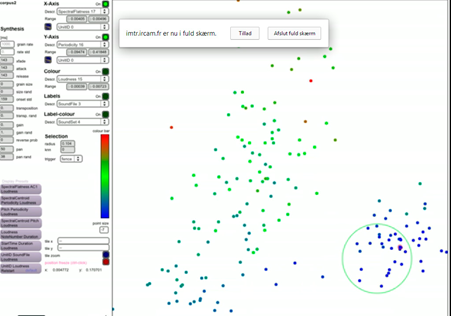
\includegraphics[height=5cm]{fig/cataRT.png}
		\caption{cataRT picture form video of cataRT showing the interface. http://imtr.ircam.fr/imtr/CataRT}
		\label{cataRT}
	\end{center}
\end{figure} 
These methods could be used to make a voice imitate an instrument if a database was to be made with a given instrument, then by using this method it will be possible to analyze the input voice and find the closets sound from the database of the instrument sounds. Some analysis criteria would be needed to find the right database sound e.g. the pitch. 

 				  = = = = = = = = = = = =

\subsection{ Software to transcribe instruments }
Since “modern beatboxing” evolved, it seems like technology is reclaiming it is technological importance. Some artists are beginning to transcribe instruments, adding filters and effects to beatboxing which takes the complexity of beatboxing even further. I.e. Dub FX, Benjamin Stanford from Australia, who samples sequences of vocal basslines, grooves and adds effects to them. Lately he re-recorded ‘Love Someone’ using Roland RC-505, a so called ‘Loop Station’, based on sequential recording of each track in instrumental compositions. [2] This way, he can perform on streets as one person, sounding as an orchestra. ** NEED TO WRITE MORE ON TRANSCRiPTION**